\documentclass[11pt,a4paper]{article}
\usepackage[utf8]{inputenc}
\usepackage[T1]{fontenc}
\usepackage[french]{babel}
\usepackage[a4paper,margin=2cm]{geometry}
\usepackage{graphicx}
\usepackage{amsmath,amssymb}
\usepackage{booktabs}
\usepackage{array}
\usepackage{float}
\usepackage{caption}
\usepackage{enumitem}
\usepackage{xcolor}
\usepackage[hidelinks]{hyperref}

\captionsetup{font=small,labelfont=bf}
\setlist{nosep,leftmargin=1.4em}
\setlength{\parskip}{2pt}
\setlength{\parindent}{0pt}

\title{\vspace{-1.2cm}\textbf{Optimisation hivernale : tournées de déneigement à Montréal}}
\author{Projet ERO1 — Groupe 10 (APPING1)}
\date{\vspace{-0.4cm}}

\begin{document}
\maketitle
\vspace{-0.6cm}

\begin{abstract}\small
\noindent Nous optimisons les tournées des déneigeuses sur quatre arrondissements de
Montréal (Outremont, Verdun, Anjou, Rivière-des-Prairies–Pointe-aux-Trembles).
Le réseau routier est modélisé comme un graphe orienté ; déneiger toutes les
rues à coût minimal est le \emph{problème du postier chinois dirigé}, que nous
résolvons par un \emph{flot à coût minimum} suivi de l'extraction d'un circuit
eulérien. Nous comparons trois scénarios de priorisation (axes structurants,
services essentiels, coût minimal) au moyen d'indicateurs génériques et
spécifiques, et nous en analysons l'impact à l'aide d'une matrice éthique.
\end{abstract}

\section{Formalisation et méthode de résolution}

\subsection{Données, périmètre et contraintes}
\textbf{Données.} Le réseau routier carrossable de chaque arrondissement provient
d'OpenStreetMap (extraction via \texttt{osmnx}, type \texttt{drive}). Chaque
tronçon de rue porte sa longueur (en mètres) et son type fonctionnel
(\texttt{highway}). Les points d'intérêt sensibles (hôpitaux, écoles, casernes,
arrêts de transport) sont également extraits d'OpenStreetMap. Les paramètres
économiques sont ceux fournis par la municipalité (Tab.~\ref{tab:donnees}).

\begin{table}[H]
\centering\small
\begin{tabular}{lr@{\hspace{2em}}lr}
\toprule
Coût fixe & 500 \$/jour & Coût horaire ($\leq 8$\,h) & 1{,}1 \$/h\\
Coût kilométrique & 1{,}1 \$/km & Coût horaire ($>8$\,h) & 1{,}3 \$/h\\
Vitesse moyenne & 10 km/h & Seuil heures sup. & 8 h\\
\bottomrule
\end{tabular}
\caption{Données municipales utilisées (par déneigeuse).}
\label{tab:donnees}
\end{table}

\textbf{Périmètre et contraintes retenues.} (i)~\emph{Couverture totale} : toute
rue du secteur doit être déneigée au moins une fois. (ii)~\emph{Sens de
circulation} : les rues à sens unique sont des arcs orientés ; le code de la
route est respecté (pas de marche arrière). (iii)~\emph{Priorisation} : certains
tronçons sont traités avant d'autres selon le scénario. (iv)~\emph{Coût et
durée} : on intègre le seuil d'heures supplémentaires (8\,h) et la vitesse
moyenne. \textbf{Hors périmètre} (hypothèses simplificatrices) : on ne modélise
ni l'épandage de sel, ni le chargement/évacuation de la neige, ni la congestion
variable, ni la largeur des voies ; une déneigeuse traite une voie par passage.

\subsection{Hypothèses de modélisation}
\begin{itemize}
\item Une rue est \emph{déneigée} dès le premier passage de la déneigeuse (elle
dégage la voie en roulant) ; les passages suivants sont des déplacements
« à vide » (\emph{deadhead}).
\item Vitesse constante (10 km/h) : la durée est proportionnelle à la distance.
\item Les déneigeuses partent et reviennent à un même dépôt ; elles sont
identiques.
\item Le réseau de chaque secteur est ramené à sa plus grande composante
fortement connexe (garantit l'existence d'un circuit), ce qui couvre la quasi
totalité de la voirie.
\end{itemize}

\subsection{Formalisation : du postier chinois au flot à coût minimum}
On modélise le secteur par un graphe orienté $G=(V,A)$ où $V$ est l'ensemble des
intersections et $A$ l'ensemble des tronçons de rue ; chaque arc $a=(i,j)$ a une
longueur $w_a>0$. Déneiger toute la ville à distance minimale revient à trouver
un \textbf{parcours fermé empruntant chaque arc au moins une fois}, de longueur
totale minimale : c'est le \emph{postier chinois dirigé}~\cite{edmonds1973}.

Un graphe orienté connexe admet un \textbf{circuit eulérien} (passant une et une
seule fois par chaque arc) si et seulement si, en chaque nœud, le degré entrant
égale le degré sortant. Notre graphe ne vérifie pas cette propriété : il faut
\emph{ajouter} le minimum de passages supplémentaires pour rééquilibrer les
degrés. Soit $x_a\in\mathbb{N}$ le nombre de passages \emph{supplémentaires} sur
l'arc $a$ (l'arc est parcouru $1+x_a$ fois). En notant $\delta^+(i)$ et
$\delta^-(i)$ les arcs sortant/entrant de $i$, le problème s'écrit :
\begin{equation}
\min_{x\ge 0}\ \sum_{a\in A} w_a\, x_a
\quad\text{s.c.}\quad
\sum_{a\in\delta^-(i)} x_a-\!\!\sum_{a\in\delta^+(i)} x_a = b_i\ \ \forall i\in V,
\qquad b_i=\deg^+(i)-\deg^-(i).
\label{eq:mcf}
\end{equation}
Le terme $b_i$ est le \emph{déséquilibre} du nœud $i$. Le programme
\eqref{eq:mcf} est exactement un \textbf{problème de flot à coût minimum} (vu en
cours) : on « expédie » des passages supplémentaires des nœuds en excès de
sortie vers les nœuds en excès d'entrée, au coût de la longueur des rues
empruntées. Comme $\sum_i b_i=0$ et que les $b_i$ sont entiers, la solution est
entière. Le multigraphe formé des rues (une fois) et des $x_a$ duplications est
alors eulérien : on en extrait un circuit par l'algorithme de Hierholzer.

\subsection{Méthode retenue et alternatives}
Le tableau~\ref{tab:methodes} résume les méthodes envisagées. Nous retenons la
réduction \textbf{flot à coût minimum + circuit eulérien} : elle est
\emph{exacte} pour le postier chinois dirigé, s'appuie directement sur les
outils du cours, et passe à l'échelle (résolution $<1$\,s sur
Rivière-des-Prairies, 5\,191 arcs).

\begin{table}[H]
\centering\small
\begin{tabular}{p{4.4cm}p{4.0cm}p{6.2cm}}
\toprule
Méthode & Adéquation & Décision\\
\midrule
Plus court chemin (Dijkstra) & relie deux points & insuffisant : ne couvre pas \emph{toutes} les rues\\
Voyageur de commerce (TSP) & visite des \emph{sommets} & inadapté : on couvre des \emph{arcs}, pas des nœuds ; NP-difficile\\
\textbf{Postier chinois dirigé via flot à coût min.} & couvre tous les arcs, sens uniques & \textbf{retenue} : exacte, alignée au cours, rapide\\
Postier rural dirigé & couvre un \emph{sous-ensemble} d'arcs & retenue pour les passes prioritaires (S1, S2)\\
\bottomrule
\end{tabular}
\caption{Recherche et choix de la méthode de résolution au vu du contexte.}
\label{tab:methodes}
\end{table}

Pour les scénarios priorisés, on couvre d'abord un sous-ensemble de rues : c'est
le \emph{postier rural dirigé}, résolu par la même mécanique (connexion des
composantes par plus courts chemins, rééquilibrage par flot à coût minimum,
circuit eulérien). Pour la \textbf{flotte} de $k$ véhicules, on applique une
heuristique « route d'abord, découpe ensuite » : la tournée d'un véhicule est
découpée en $k$ tronçons de longueur égale, chacun relié au dépôt par un plus
court chemin.

\subsection{Indicateurs génériques}
Pour toute solution : distance totale parcourue (km), part de déplacements à vide
(\%), durée et coût total (\$), et \emph{temps de remise en service} d'une classe
de rue = instant où le dernier tronçon de cette classe est déneigé.

\subsection{Limites du modèle}
La vitesse constante ignore la congestion et la météo ; le découpage de flotte
est heuristique (borne supérieure, non optimale) ; les passes prioritaires
engendrent des déplacements à vide importants (cf. §3) ; un seul dépôt est
considéré ; le déneigement est supposé instantané au passage (pas de file
d'attente de chargement). Ces limites sont acceptables pour comparer des
\emph{scénarios} à l'échelle d'une journée type.

\section{Trois scénarios de priorisation}
Les trois scénarios traitent l'\textbf{intégralité} de la voirie ; ils diffèrent
par l'\emph{ordre} de traitement. La priorisation repose sur la classification
fonctionnelle des rues (axes structurants, voies collectrices, desserte locale)
et sur la proximité des services essentiels.

\paragraph{S1 — Axes d'abord (fluidité du trafic).} On déneige d'abord les axes
structurants, puis les collectrices, puis la desserte locale. \emph{Argumentaire}
: la politique réelle de la Ville de Montréal traite en priorité le réseau
artériel et les circuits d'autobus pour éviter la paralysie économique~\cite{vdm,new18}.
\emph{Bénéfices / cibles} : automobilistes, transport collectif, activité
économique ; remise en circulation rapide des grands axes. \emph{Risques} :
les rues résidentielles et certains services restent enneigés longtemps ;
déplacements à vide accrus. \emph{Indicateur} : temps de remise en service des
axes structurants.

\paragraph{S2 — Services essentiels (sécurité et accès).} On déneige d'abord les
rues bordant hôpitaux, écoles, casernes et arrêts de transport. \emph{Argumentaire}
: l'accès des secours et des populations vulnérables est un objectif de sécurité
publique reconnu~\cite{vdm}. \emph{Bénéfices / cibles} : patients, élèves,
personnes à mobilité réduite, services d'urgence. \emph{Risques} : services
dispersés $\Rightarrow$ déplacements à vide très élevés et coût accru ; le reste
du réseau est déneigé tardivement. \emph{Indicateur} : temps de remise en service
des rues « services essentiels ».

\paragraph{S3 — Coût minimal (référence budgétaire).} Aucune priorité : on
minimise directement la distance (postier chinois pur). \emph{Argumentaire} : la
pression budgétaire sur le déneigement est un enjeu récurrent à Montréal~\cite{lef19,vezina20}.
\emph{Bénéfices / cibles} : contribuables, équilibre du budget municipal.
\emph{Risques} : aucune garantie de service pour les axes ni les services
sensibles ; équité non prise en compte. \emph{Indicateur} : coût total et
distance à vide.

\subsection{Analyse d'impact : matrice éthique}
La matrice éthique~\cite{mepham2006} croise les parties prenantes et trois
familles de valeurs : \emph{bien-être} (utilitarisme), \emph{autonomie}
(déontologie) et \emph{justice} (équité). Le tableau~\ref{tab:ethique} fait
apparaître les tensions propres à chaque scénario.

\begin{table}[H]
\centering\small
\renewcommand{\arraystretch}{1.15}
\begin{tabular}{p{2.6cm}p{4.1cm}p{4.0cm}p{4.0cm}}
\toprule
Partie prenante & Bien-être & Autonomie & Justice\\
\midrule
Automobilistes / éco. & \textbf{S1+} axes dégagés vite ; \textbf{S2/S3$-$} trafic ralenti & S1 favorise la mobilité motorisée & S1 avantage le transit au détriment du local\\
Riverains résidentiels & \textbf{S1/S2$-$} rues locales déneigées en dernier & subissent l'ordre choisi sans consultation & \textbf{S3$+$} traite tout le monde « pareil », mais tard\\
Pop. vulnérables / secours & \textbf{S2+} accès hôpitaux/écoles prioritaire & meilleure capacité d'accès aux soins & \textbf{S2+} corrige une inégalité d'accès\\
Municipalité / contribuables & \textbf{S3+} coût minimal ; \textbf{S2$-$} coût élevé & marge budgétaire préservée (S3) & arbitrage coût/équité à assumer\\
\bottomrule
\end{tabular}
\caption{Matrice éthique des trois scénarios ($+$ effet favorable, $-$ défavorable).}
\label{tab:ethique}
\end{table}

\section{Analyse des résultats}
On illustre sur \textbf{Anjou} (220{,}6 km de voirie, seul secteur réunissant les
trois classes de rues), puis on généralise aux quatre secteurs.

\begin{table}[H]
\centering\small
\begin{tabular}{lrrrrrr}
\toprule
& Dist. & À vide & Coût/véh & Axes & Essentiels & Fin\\
Scénario (Anjou) & (km) & (\%) & (\$) & dégagés & dégagés & secteur\\
\midrule
S1 — Axes d'abord & 362 & 64 & 944 & \textbf{3{,}6 h} & 35{,}6 h & 35{,}7 h\\
S2 — Services essentiels & 400 & 81 & 990 & 39{,}8 h & \textbf{16{,}4 h} & 39{,}8 h\\
S3 — Coût minimal & \textbf{265} & \textbf{20} & \textbf{824} & 26{,}4 h & 26{,}4 h & \textbf{26{,}4 h}\\
\bottomrule
\end{tabular}
\caption{Indicateurs génériques et spécifiques (Anjou, 1 véhicule de référence).}
\label{tab:anjou}
\end{table}

\textbf{Lecture (Tab.~\ref{tab:anjou}, Fig.~\ref{fig:compromis}).} S3 minimise le
coût (824 \$, seulement 20\,\% à vide) mais ne dégage rien en avance : tout est
traité à 26{,}4 h. S1 dégage les axes en \textbf{3{,}6 h} (dix fois plus vite),
au prix de $+15\,\%$ de coût et de 64\,\% de déplacements à vide. S2 dégage les
services essentiels en \textbf{16{,}4 h} (contre 26{,}4 h en S3), mais c'est le
plus coûteux (990 \$, 81\,\% à vide) car les services sont géographiquement
dispersés. Chaque scénario optimise donc une dimension différente : il n'existe
pas de solution dominant les autres.

\begin{figure}[H]
\centering
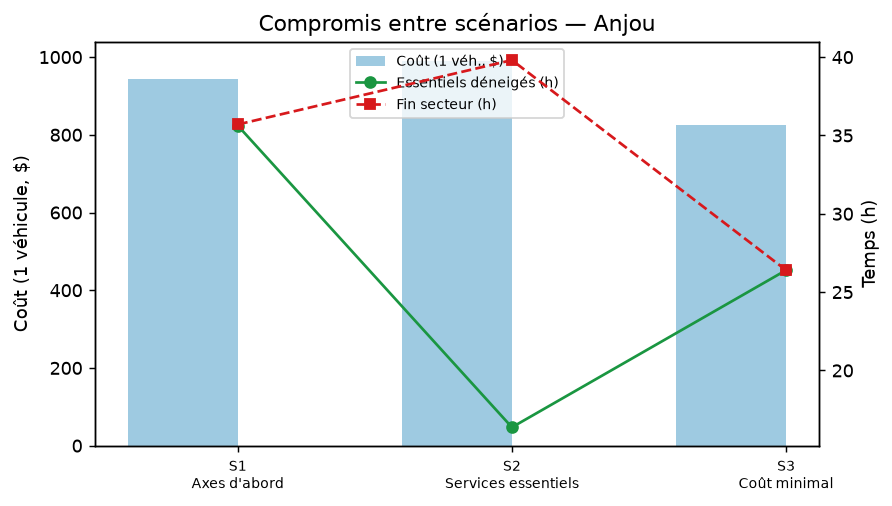
\includegraphics[width=0.49\textwidth]{figures/compromis_anjou.png}
\hfill
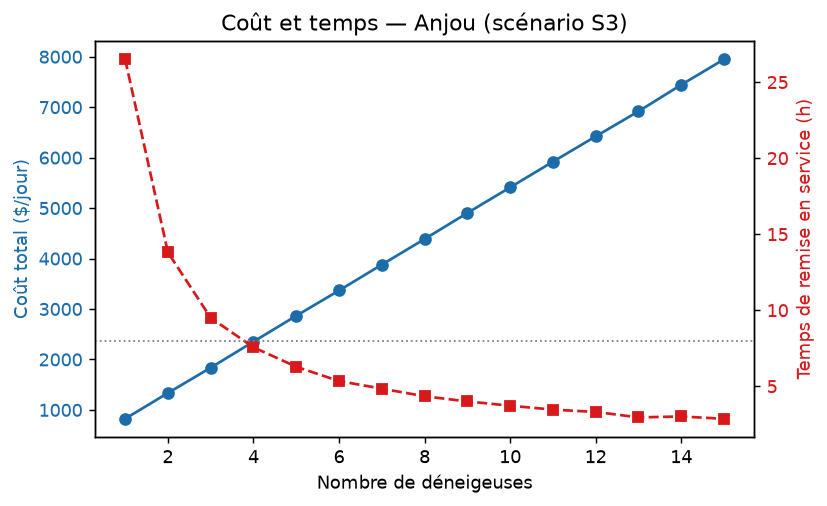
\includegraphics[width=0.49\textwidth]{figures/cout_vehicules_anjou.png}
\caption{À gauche : compromis coût / temps de remise en service par scénario
(Anjou). À droite : coût total et temps de remise en service en fonction du
nombre de déneigeuses (scénario S3). Le temps passe sous 8 h à partir de 4
véhicules.}
\label{fig:compromis}
\end{figure}

\textbf{Modèle de coût et dimensionnement de la flotte.} Avec une seule
déneigeuse, le secteur d'Anjou demanderait $\approx 26$ h : irréaliste. La
courbe coût $=f(\text{nombre de véhicules})$ (Fig.~\ref{fig:compromis}, droite)
montre un coût qui croît linéairement (le coût fixe de 500 \$/véhicule domine)
et un temps qui décroît en $1/k$. Le plus petit effectif respectant la borne de
8 h est de \textbf{4 véhicules} (7{,}6 h, 2\,353 \$/jour). Le
tableau~\ref{tab:synthese} étend ce dimensionnement aux quatre secteurs.

\begin{table}[H]
\centering\small
\begin{tabular}{lrrrr}
\toprule
Secteur & Voirie (km) & Tournée S3 (km) & Flotte ($\leq$8 h) & Coût/jour (\$)\\
\midrule
Outremont & 70 & 81 & 2 & 1\,103\\
Verdun & 102 & 110 & 2 & 1\,145\\
Anjou & 221 & 265 & 4 & 2\,353\\
Rivière-des-Prairies–P.-a.-T. & 707 & 786 & 13 & 7\,634\\
\midrule
\textbf{Total (4 secteurs)} & \textbf{1\,100} & \textbf{1\,242} & \textbf{21} & \textbf{12\,235}\\
\bottomrule
\end{tabular}
\caption{Dimensionnement de la flotte par secteur (scénario S3, remise en
service $\leq 8$ h). La part de déplacements à vide reste faible en S3
(8–20 \%).}
\label{tab:synthese}
\end{table}

\begin{figure}[H]
\centering
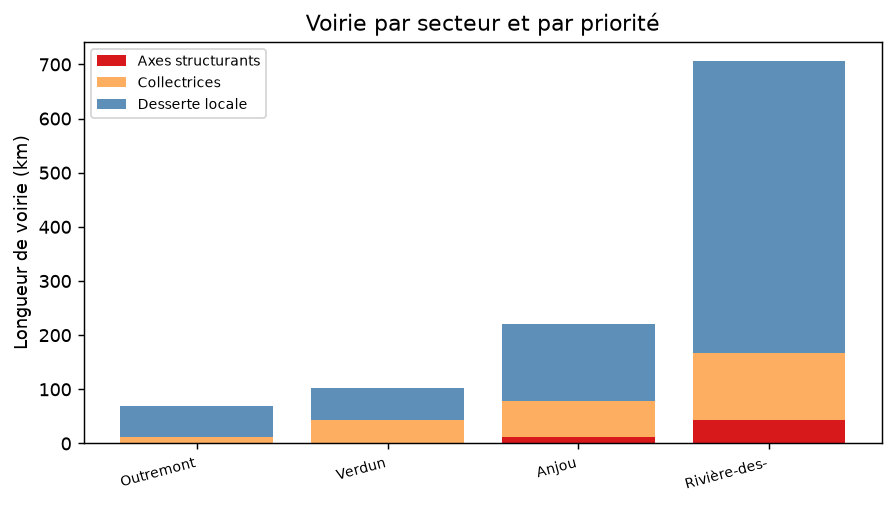
\includegraphics[width=0.40\textwidth]{figures/voirie_par_secteur.png}
\hfill
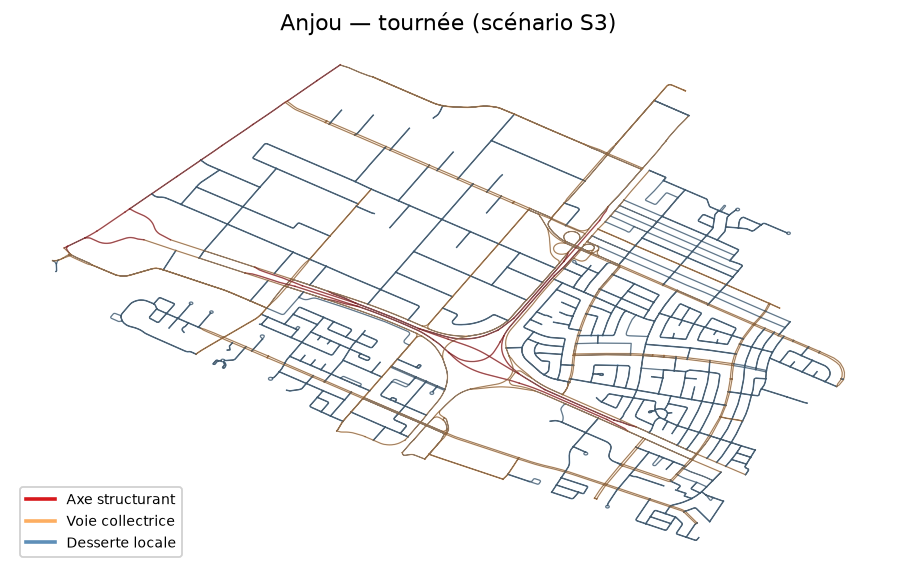
\includegraphics[width=0.56\textwidth]{figures/carte_anjou.png}
\caption{À gauche : longueur de voirie par secteur et par classe de priorité.
À droite : réseau d'Anjou coloré par priorité (rouge = axes, orange =
collectrices, bleu = desserte locale) avec la tournée du scénario S3.}
\label{fig:carte}
\end{figure}

\subsection{Projection des effets réels sur les habitants}
\textbf{S1 (axes d'abord).} \emph{Positif} : remise en circulation rapide des
grands axes et des lignes de bus — l'activité économique et les déplacements
pendulaires reprennent vite ; les véhicules d'urgence circulent mieux sur le
réseau structurant. \emph{Négatif} : les rues résidentielles restent enneigées
très longtemps (desserte locale dégagée en dernier) et, paradoxalement, les
abords de certains services (écoles de quartier) attendent ; injustice spatiale
au détriment des quartiers purement résidentiels.

\textbf{S2 (services essentiels).} \emph{Positif} : un patient, un élève ou une
personne à mobilité réduite accède aux services et aux secours nettement plus
tôt (16 h contre 26 h) ; gain d'équité et de sécurité. \emph{Négatif} : le coût
le plus élevé (jusqu'à 81\,\% de déplacements à vide) pèse sur le budget, et le
reste du réseau est déneigé tardivement — la majorité des usagers « ordinaires »
attend plus longtemps. Le bénéfice se paie en argent public et en délai pour le
plus grand nombre.

\textbf{S3 (coût minimal).} \emph{Positif} : déneigement le moins cher, le plus
sobre (moins de kilomètres parcourus, donc moins d'émissions et d'usure) ;
traitement « égalitaire » de toutes les rues. \emph{Négatif} : aucune garantie
de service — un axe vital ou l'accès à un hôpital peut n'être dégagé qu'en toute
fin de tournée ; en cas d'épisode intense, le risque sanitaire et économique
n'est pas maîtrisé.

\subsection{Critique et recommandation}
Aucun scénario n'est globalement supérieur : S3 est \emph{efficient} mais
\emph{aveugle au service}, S1 sert la mobilité mais néglige l'équité, S2 sert
l'équité mais coûte cher et retarde la majorité. En pratique, une politique
\emph{hybride} — services essentiels et axes structurants en première vague,
puis desserte locale au coût minimal — combinerait l'essentiel des bénéfices ;
notre outil permet d'en chiffrer le compromis. La forte part de déplacements à
vide des scénarios priorisés (heuristique de postier rural) constitue une borne
supérieure : un solveur de tournées plus fin la réduirait, ce qui resserrerait
l'écart de coût avec S3 sans changer l'ordre des conclusions.

\begin{thebibliography}{9}\small
\bibitem{edmonds1973} J.~Edmonds, E.~L.~Johnson. \emph{Matching, Euler tours and
the Chinese postman}. Mathematical Programming, 1973.
\bibitem{eiselt1995} H.~A.~Eiselt, M.~Gendreau, G.~Laporte. \emph{Arc routing
problems}. Operations Research, 1995.
\bibitem{vdm} Ville de Montréal. \emph{Tout savoir sur le déneigement dans
l'arrondissement}. Opération déneigement.
\bibitem{new18} CBC News. \emph{How Montreal takes 300\,000 truckloads of snow
off the street every winter}, 2018.
\bibitem{lef19} S.-M.~Lefebvre. \emph{Les prix du déneigement explosent partout
au Québec}. Journal de Montréal, 2019.
\bibitem{vezina20} H.~Ouellette Vézina. \emph{Déneigement : « on craint toujours
de dépasser le budget »}. Métro, 2020.
\bibitem{mepham2006} B.~Mepham, M.~Kaiser, E.~Bjørnerud, S.~Tomkins.
\emph{Ethical Matrix Manual}, 2006.
\end{thebibliography}

\end{document}
